\documentclass[a4paper, oneside]{book}

\bibliographystyle{IEEEtran}
%\usepackage{cite}

%% Language and font encodings
\usepackage[english]{babel}
\usepackage[utf8x]{inputenc}
\usepackage[T1]{fontenc}

% Palatino for rm and math | Helvetica for ss | Courier for tt
\usepackage{mathpazo} % math & rm
\linespread{1.05}        % Palatino needs more leading (space between lines)
\usepackage[scaled]{helvet} % ss
\usepackage{courier} % tt
\normalfont
\usepackage[T1]{fontenc}

%% Sets page size and margins
\usepackage[a4paper,top=3cm,bottom=2cm,left=3cm,right=3cm,marginparwidth=1.75cm]{geometry}

%% Useful packages
\usepackage{amsmath}
\usepackage{longtable,array}
\newcounter{ltrow}
\usepackage{float}
\usepackage[colorinlistoftodos]{todonotes}
\usepackage[colorlinks=false, allcolors=blue]{hyperref}
\usepackage{graphicx}
\graphicspath{ {images/} }
\usepackage{rotating}
\usepackage{enumitem}
\usepackage[titletoc]{appendix}

%% Custom settings
\setlength\parindent{0pt}

%% Title and author
\title{
    {\textbf{Analyzing Recurrent Neural Networks based on Visually Grounded Speech signals: encoding of speaker identity}}\\
    \vspace{2cm}
	{
	\begin{figure}[h]
	\centering
	
\includegraphics[scale=0.15]{images/Tilburg_University_logo.png}\\
	\end{figure}
	}
}
\author{
Master's thesis \\
Communication and Information Sciences \\
Specialization track Data Science: Business and Governance \\
Tilburg University - School of Humanities \\\vspace{1cm}\\
Mark van der Laan \\ 
\textit{\href{mailto:m.l.vdrlaan@tilburguniversity.edu}{m.l.vdrlaan@tilburguniversity.edu}} \\ ANR: 633762 \\\vspace{1cm}\\ 
Supervisor: dr. G. ChrupaŁa \\ 
Second reader: dr. D. Hendrickson}

\begin{document}

\maketitle
\chapter*{Abstract}

This thesis presents research on how the unique characteristics of voice are encoded in a Recurrent Neural Network (RNN) trained on Visually Grounded Speech signals. Multiple experiments were performed in order to determine if and to what extent speaker identity is encoded. These experiments were executed against raw MFCC vectors, a convolutional layer and the recurrent layers of the neural network. This thesis also describes the process of labeling gender in both the Flickr8K and the Places 205 audio caption dataset. \\

The most important takeaway is that the presented model identifies speakers and classify their gender based on manually labelling of both datasets. Moreover, encoding of speaker identification and gender are most prevalent in the first few layers of the neural network. This finding aligns with the research that has been done on encoding of phonemes in this type of model: ‘form-related aspects’ are most prevalent in the first few layers while semantics are better encoded in the deeper layers. Experiments regarding gender classification reveal that there is a difference in accuracy between male and female (gender bias). The gender bias experiment shows that, contrary to the recurrent layers, the raw MFCC vectors and convolutional layer indeed have accuracy difference between gender. 

\chapter*{Preface}

This thesis is written to fulfill the master program of Data Science: Business and Governance which is a specialization track within the master program of Communication and Information Sciences. \\

I would like to thank my supervisor dr. Gregorz Chrupa\l a for all the work he has done to make the execution of this thesis possible and the valuable feedback that he gave me. With help of dr. Chrupa\l a the Neural Network presented in \autoref{chapter:methods-and-datasets} was trained so that I could use the output to execute this thesis. Besides, I also would like to thank Alessandro Hazenberg for helping me to label the data and my family for their support. \\

Yours sincerely,
\begin{figure}[H]

\includegraphics[scale=0.1]{images/sign.png}
\end{figure}
Mark van der Laan \\
\textit{Tilburg \today}

\tableofcontents

\listoftables

\listoffigures

% CHAPTER INTRODUCTION
\chapter{Introduction}\label{chapter:introduction}

The scientific field of computational linguistics is concerned with finding methods to systematically and algorithmically acquire important characteristics of natural language like syntax and semantics. A subfield of computational linguistics is speaker recognition which can be defined as: \textit{‘extract, characterize and recognize the information in the speech signal conveying speaker identity’} \cite{reynolds2002overview}. Within the field of speaker recognition multiple facets are researched like speaker identification (i.e. identify a speaker from a known set of speakers), speaker verification (i.e. reject the identity of the speaker based on the provided signal) and speaker diarisation (i.e. identify speakers in speech signals with multiple speakers) \cite{reynolds2002overview} \cite{tranter2006overview}. \\

Within the subfield of speaker recognition, this thesis mainly focuses on speaker identification. More specifically, speaker identification is researched within the context of neural networks trained on Visually Grounded Speech signals. This type of neural network is trained on visual (i.e. images) and auditory input (i.e. spoken captions) to learn syntax and semantics from continuous speech. Contrary to older methods, like using text transcriptions, this method requires less supervision and it becomes possible to learn language-independent \cite{HarwathG15}. From a societal perspective this is interesting because with this method less spoken languages can also be analyzed on their syntax and semantics. Moreover, some spoken dialects do not have a specific writing system so methods based on text transcriptions cannot encode these spoken dialects. \\

Within the context of neural networks based on Visually Grounded Speech signals it is currently not known how speaker identification is encoded. Therefore, the research question for thesis is: \\

\textit{‘How will speaker identity be encoded in Recurrent Neural Networks based on Visually Grounded Speech signals?’} \\


Previous work looked into this type of neural network to see how phonemes are encoded. Researchers \cite{AlishahiBC17} found out that phoneme encoding follows a certain pattern which is that ‘form-related aspects’ are more prevalent in the first few layers of the neural network while all the semantic information is better encoded in the deeper layers. The hypothesis for this research question is that speaker identification also follows this pattern. This implies that the first layers encode speakers better due to the fact that speaker identification is a form-related aspect. This finding aligns with the general understanding of deep neural networks which presumes that deeper layers can learn more complex patterns \cite{lecun2015deep}. \\

In \autoref{chapter:background}, I present information that is relevant to this thesis, like the work that already has been done on this type of neural network. After providing background information, it is important to explain the most important characteristics of the data and the type of models that are used throughout this thesis which is presented in \autoref{chapter:methods-and-datasets}. Based on the data and the model type, experiments are executed which are presented in \autoref{chapter:experiments}. This thesis will end with a brief overview of possible future work and a concise conclusion.

% CHAPTER BACKGROUND
\chapter{Background}\label{chapter:background}

In this chapter I will provide background information and previous established work that is relevant to this thesis. In \autoref{background:speaker-identification} I will provide an overview of what already has been done on the automatic identification of speakers. In \autoref{background:visually-grounded-speech} previous work on Visually Grounded Speech is provided while \autoref{background:gender-bias-in-machine-learning} gives an overview of literature that considered gender bias in Machine Learning.

\section{Speaker identification}\label{background:speaker-identification}
The first attempts of speech recognition date back to at least the seventies of the previous century \cite{huang2014historical}. The urge for speaker recognition systems came from different disciplines like law enforcement (e.g. monitoring prison calls), access control (e.g. give access to a system based on voice verification) and technology firms (e.g. personalize web content)  \cite{reynolds2002overview}. The performance of first generation speech recognition systems were hindered by constraints that occurred during that era like limited computational power, lack of understanding how to cancel out background noise and lack of advanced models like neural networks or support vector machines \cite{huang2014historical}. \\

Systems specifically concerned with the task of identifying speakers from a known set of speakers date back at least to the 

\section{Visually Grounded Speech}\label{background:visually-grounded-speech}
Models with speech and text transcriptions have been a popular method in Machine learning to learn from speech signals \cite{HarwathG15}. In \cite{HarwathG15} presents a model which substitutes the text transcriptions with relevant images. This methodology requires less supervision than text transcriptions because it is not possible to analyze the speech orthographically (i.e. using a writing system). This makes it harder to analyze and extract linguistic constructs because the same word pronounced by different speakers can adhere differences in the analysis. Therefore they decided to only train the model on words instead of whole sentences in order to reduce the complexity. The conclusion of this research is that a model focused on learning words with speech and accompanying images can learn syntax and semantics on word-level. An interesting factor is that this way of learning resembles the way humans learn more closely because humans are enabled to learn by just grounding stimuli in their sensory environment. \\

In \cite{harwath2016unsupervised} they also developed a model based on Visually Grounded Speech signals and extended this idea. Contrary to \cite{HarwathG15}, this research focuses on continuous speech signals instead of just words. Like \cite{HarwathG15}, \cite{harwath2016unsupervised} grounds images and speech signals by mapping the modalities in the same semantic space, where a pair that describes the same scene has a higher similarity score than a pair which does not describe the same thing. This research revealed that the model can learn from continuous speech and can also learn semantic information. \\

In \cite{HarwathG15} and \cite{harwath2016unsupervised} a convolutional architecture is used to train the model. Speech signals that weren't the same length were padded with zeros. In \cite{ChrupalaGA17} they also used images and continuous speech directly but instead of a convolutional architecture, a recurrent multi-layer architecture was used. This recurrent multi-layer architecture performs better than the previously proposed convolutional architecture. Research also revealed how the different layers encode information regarding syntax and semantics. They found that form-related aspects (e.g. how different speakers pronounce the same word) and semantics (e.g. identifying which words are important in a sentence) are better encoded in different parts of the neural network. \\

In \cite{AlishahiBC17} they use this recurrent multi-layer architecture to analyze how phonemes are encoded. The model is trained on synthetic speech from the Microsoft Common Objects in Context (MS COCO) dataset. The results of the executed experiments, like phoneme decoding and phoneme discrimination, aligned with what has been found in \cite{ChrupalaGA17} that semantics are more prevalent in the deeper layers while form-related aspects are more prevalent in the first few layers. 

\section{Gender bias in Machine Learning}\label{background:gender-bias-in-machine-learning}
Multiple characteristics of the human voice have influence on how models interpret and classify speech signals. Characteristics like gender, accent and age are important to the performance of speaker identification models \cite{abdulla2001improving}. If these characteristics are insufficiently addressed it could be possible that certain speakers have lower error rates than others. \\

In \cite{Tatman2017GenderAD} examined how accent and gender influence the results in the Automatic Speech Recognition (ASR) system of Youtube. The most important finding is that females and people from Scotland consistently obtain lower rates of accuracy than males and other accents.  Conclusions are based on a so-called ‘accent challenge’ experiment with a low amount of participants (N=80). This experiment required the participants to pronounce a list of words which can clearly discriminate between different accents within a language. \\

Research on gender bias in speaker identification is limited and it is therefore not possible to give definitive answer on why differences occur (\cite{Tatman2017GenderAD}, \cite{abdulla2001improving}). One possible reason is that there is imbalance in the data. For example, it may be the case that the model of the ASR of Youtube is trained on more male than female feature vectors. Another possible reason for bias is that there are differences in pitch between males and females \cite{latinus2012discriminating}. Pitch differences occur due to biological reasons (e.g. length of the vocal tract) and the style of the speaker which may differ between male and female \cite{meena2013gender}. The difference in pitch is a factor that may contribute to performance differences, however, in \cite{Tatman2017GenderAD} no significant effect was found. \\

Inspired by this research, an experiment in this thesis is presented which examines whether there are any performance differences between male and female in neural networks based on Visually Grounded Speech signals. There is specifically chosen for gender bias because this the only mentioned characteristic that is available for analysis. Caution must therefore be taken to interpret results because confounding variables like accent and age may influence the results. \\ 

Results in this thesis cannot directly be compared to \cite{Tatman2017GenderAD} because bias is examined in a restrained environment based on words instead of continuous speech fragments. Continuous speech fragments are substantially more subject to background noise. Moreover, the experiment in this thesis differs from \cite{Tatman2017GenderAD} because the accuracy scores are obtained through a system which focus on speech recognition. 


% CHAPTER METHODS AND DATASETS
\chapter{Methods and datasets}\label{chapter:methods-and-datasets}

This chapter specifies the specifics of the dataset and how the research is going to be validated. In \autoref{methods-and-datasets:data} there is elaborated on the key characteristics of the dataset. \autoref{methods-and-datasets:labeling-of-gender} describes the procedure that is used to label the gender of each speaker in each dataset \footnote{All the code that was used to execute the experiments and labeling the data in this thesis can be found in https://github.com/markvdlaan93/vgs-speaker-identification.}. Finally, \autoref{methods-and-datasets:models} explains which models are used and its characteristics.

\section{Data}\label{methods-and-datasets:data}

Contrary to the dataset used in \cite{AlishahiBC17}, the dataset for this thesis consists of human spoken utterances instead of synthetic speech. I started with the Flickr8K audio caption dataset \cite{HarwathG15, hodosh2013framing} which consists of 8,000 images with each five spoken captions generated by more than 180 participants in Amazon's Mechanical Turk. The Places dataset is also used in this thesis \cite{Zhou2014}. Like the Flickr8K dataset, the Places dataset also consists of human spoken utterances collected through Amazon’s Mechanical Turk but this dataset is much larger with more than 200.000 utterances and 1.400 participants and is contextually richer than the Flickr8K dataset \cite{Harwath2017LW}. This becomes clear when the audio records of the Places validation set are played: the audio records are longer, contain more words and the pauses between words are longer. \\

\section{Labeling of gender}\label{methods-and-datasets:labeling-of-gender}

To check whether a speaker is male or female, I listened for each speaker to an audio record provided in the validation dataset of Flickr8K and Places. For each speaker, to make sure no mistakes are made, the audio record is also labelled by a second listener. After the second round, the results of the first two rounds were compared and checked whether there were any differences between these two rounds. For the audio records of the speakers which didn't match in the first two rounds, another audio record is picked to determine whether the speaker is a male or female. \\ 

\section{Distribution of data}\label{methods-and-datasets:distribution-of-data}

The results of this procedure are presented in \autoref{labeling-of-gender:entries} and \autoref{labeling-of-gender:quantities}. For the Places dataset it was necessary to remove one speaker with a single entry because for some reason the audio record is not available in the package of the dataset \cite{harwath2016unsupervised} although the supplemented instructions say otherwise.

\begin{table}[H]
\begin{center}
\begin{tabular}{|l|rl|}
\hline      & \bf Flickr8K  & \bf Places \\ \hline
\bf Male    & 2.697         & 550 \\
\bf Female  & 2.303         & 449 \\ \hline
\bf Total   & 5.000         & 999 \\
\hline
\end{tabular}
\end{center}
\caption{\label{labeling-of-gender:entries} Amount of male and female speakers entries in validation sets.  }
\end{table}

\begin{table}[H]
\begin{center}
\begin{tabular}{|l|rl|}
\hline      & \bf Flickr8K  & \bf Places \\ \hline
\bf Male    & 79            & 43 \\
\bf Female  & 104           & 41 \\ \hline
\bf Total   & 183           & 83 \\
\hline
\end{tabular}
\end{center}
\caption{\label{labeling-of-gender:quantities} Amount of male and female speakers.  }
\end{table}

\section{Models}\label{methods-and-datasets:models}

This section provides an overview of the models that have I used in order to execute the experiments and see whether speaker identity and gender are encoded in the neural network. In \autoref{models:recurrent-highway-network} I will give a quick overview of the model that is used to train the data while \autoref{models:linear-models} presents the models that were used to classify each layer of the validation set.

\subsection{Recurrent Highway Network}\label{models:recurrent-highway-network}

The model which is used to train is called a so-called Recurrent Highway Network (RHN). Contrary to gated networks (e.g. Gated Recurrent Unit (GRU)), RHN’s can be used to enhance performance when recurrent depth needs to be increased \cite{ZillySKS16}. Full explanation of the model is provided in \cite{ChrupalaGA17}, I will only give a short overview here. \\ 

For a model based on Visually Grounded Speech, it is necessary to have an image and speech encoder. Together the encoders need to make sure that spoken captions and images that are related to each other do have a closer distance measure than unrelated captions and images. The distance measure in this model is the cosine similarity which calculated by the following loss function:

\begin{eqnarray}
 \sum\limits_{u, i} \Bigg( \sum\limits_{u'} max[0,\alpha + d(u,i) - d(u',i)] + \\ \nonumber
 \sum\limits_{u'} max[0,\alpha + d(u,i) - d(u,i')] \Bigg)
\end{eqnarray}

In this formula, u stands for utterance and i for image and u and i together is an image-caption pair which describe the same scene. U’ and i’ are the set of utterances and images that not describe the same scene. By taking the largest value of the subtracted cosine similarity values, the loss function delivers the image-caption pair which are the strongest related to each other. \\

The image encoder used to process the images is a pre-trained VGG-16 model \cite{Simonyan14c} which is fed with vector representations of the image. The utterance encoder has the following structure:

\begin{eqnarray}
 enc_u(\textbf{u}) = unit(Attn(RHN_k_,_L (Conv_s_,_d_,_z (\textbf{u}))
\end{eqnarray}

In this case input u consists of Mel Frequency Ceptral Coefficient (MFCC) vectors and the RHN with k recurrent layers and L depth uses the output of a convolutional layer with size s, d dimensions and stride z. The output of the RHN is fed to the attention layer which calculates the average of the activations.

\subsection{Linear models}\label{models:linear-models}

For each layer in the trained neural network (i.e. convolutional layer, recurrent layers and embedding layer) I have the mean activation values for each feature vector in the dataset to my disposal. The Flickr8K dataset has a validation set of 5,000 feature vectors and the Places validation set 1,000. The task was to feed each layer of mean activations values (i.e. matrices of 5,000 by 1,024 for Flickr8K and matrices of 1,000 by 1,024 for the Places dataset) into a linear classifier and supplement it with the labels which I also have to my disposal. This implies that the experiments in this thesis differ from training of the model because I used strongly supervised learning as opposed to the weakly supervision of Visually Grounded Speech signals. \\

The Stochastic Gradient Descent (SGD) classifier of the Python Scikit-Learn package is used in conjunction with Grid Search and Cross Validation. In \autoref{linear-models:hyperparameter-optimization} an overview is given of the parameters that I used to tune each layer. For the loss function I tried 'log' which gives Logistic Regression and 'Hinge' which gives a linear Support Vector Machine. Because of limited computational resources I decided to minimize Cross Validation only to three folds for each layer for each model. 

\begin{table}[H]
\begin{center}
\begin{tabular}{|l|r|}
\hline              & \bf Values                        \\ \hline
\bf Learning rate   & 0.01, 0.001, 0.0001 and 0.00001   \\ \hline
\bf Loss function   & Log and Hinge                     \\ \hline
\bf Penalty         & $L_{1}$, $L_{2}$ and ElasticNet   \\ 
\hline
\end{tabular}
\end{center}
\caption{\label{linear-models:hyperparameter-optimization} Values used in Grid Search in conjunction with K-fold Cross Validation.  }
\end{table}


% CHAPTER EXPERIMENTS
\chapter{Experiments}\label{chapter:experiments}

In this chapter an overview is provided of the experiments that are executed to see if and to what extent speaker identity is encoded in the proposed neural network. In \autoref{experiments:experimental-setup} I explain every aspect that is relevant to executing the experiments. After that I will present the results of each experiment in \autoref{experiments:results} and discuss these results in \autoref{experiments:discussion}.

\section{Experimental setup}\label{experiments:experimental-setup}

In \autoref{models:linear-models} I explained that each layer is trained with 3-fold Cross Validation in conjunction with Grid Search. To verify whether the model generalizes well, I decided to first split the data into a train and test set. The training set was internally split by Scikit-learn into stratified partitions of equal length. This means that this method accounts for classes imbalances presented in \autoref{methods-and-datasets:distribution-of-data}. After training the data with Cross Validation and tuning the parameters the model is trained again but this time on the entire dataset. This methodology is used for each layer for each model and the code for running the experiments is partially taken from the Scikit-learn documentation \cite{scikitlearn2017}. 

\subsection{Splitting of the datasets}\label{experimental-setup:splitting-of-the-datasets}

To account for the small size of the Places dataset (i.e. each layer consists of more dimensions than feature vectors), I decided to split the train and test set in a 60\%/40\% proportion. Because the amount of feature vectors is substantially larger for the Flickr8K dataset, I decided to split the experiments on the Flickr8K into 67\% for the training set on the remaining part for the test set (i.e. 33\%). 

\subsection{Stratification}\label{experimental-setup:stratification}

By default the train and test split function of Scikit-learn is not stratified \cite{scikitlearntraintestsplit}. Due to time constraints I decided to not stratify the classification of speaker identity on both the Flickr8K and Places dataset. The train and test split function can only be used in stratification mode when each class in dataset has at least two members. For gender classification this is not a problem because each class (i.e. male and female) has at least two members so no extra pre-processing is required. For speaker identification, this would require me to do more preprocessing which I did not have time for anymore. However, I checked whether leaving in single entries were considered in the calculation of the evaluation metrics like the accuracy and F1-score. Internally Scikit-learn ignores these observations by giving them a zero as score and not consider the single entry speakers in averaging the evaluation metric over the classes. 

\subsection{Gender bias}\label{experimental-setup:gender-bias}

To examine if the presented neural network suffers from performance differences between males and females, it was not necessary to create a separate model for each layer in each dataset. The accuracy and F1-scores per gender are derived from the classification on gender.

\subsection{Evaluation metrics}\label{experimental-setup:evaluation-metrics}

The Grid Search Cross Validation function of Scikit-learn only has the possibility to provide a single scoring function. I have decided to use the parameter ‘f1\_weighted' which calculates the F1-score per class and average the results based on the amount of instances in a certain class \cite{scikitlearn20172}. In \autoref{methods-and-datasets:distribution-of-data} I explained that I will provide both accuracy and F1-scores of each experiment. However, since the scores on the training folds will be F1-scores, I take this metric as guideline for interpreting the results. If there is any notable difference between the F1-score and accuracy for a layer, I will mention that.

\section{Results}\label{experiments:results}

For each proposed experiment I will provide the results in this section. \autoref{results:speaker-identification-in-flickr8k-dataset} starts with explaining observations for speaker identification on the Flickr8K data while \autoref{results:speaker-identification-in-places-dataset} focuses on speaker identification in the Places dataset. \autoref{results:gender-identification-in-flickr8k-dataset} and \autoref{results:gender-identification-in-places-dataset} elaborates on gender classification and \autoref{results:gender-bias} will provide results for the research regarding gender bias.

\subsection{Speaker identification in Flickr8K dataset}\label{results:speaker-identification-in-flickr8k-dataset}

In \autoref{table:speaker-identification-on-flickr8k-dataset} an overview is given of the optimal parameters for each layer. For each layer the optimal loss function, penalty and learning rate are presented. The column ‘Average training F1-score’ specifies the average F1-score over each fold for the optimal parameters. The standard deviation is an important indicator which provides insights in how consistent the predictions are over the different folds. For speaker identification in the Flickr8K dataset \autoref{table:speaker-identification-on-flickr8k-dataset} shows that the standard deviation is small (not greater than 0.04). This overview also shows that for each layer $L_{2}$ normalization gave the best results for regularization. \\

In \autoref{table:gender-speaker-classification} the performance of each experiment is presented. For speaker identification in Flickr8K dataset the classification on the raw MFCC vectors and the convolutional layer consists of approximately the same results which is followed by a sharp increase in the first recurrent layer. After the first recurrent layer the performance drops steadily till the point that the fourth recurrent layer and embedding layer are performing even worse than the raw MFCC vectors and the convolutional layer. 

\subsection{Gender identification in the Flickr8K dataset}\label{results:gender-identification-in-flickr8k-dataset}

Similar to the results presented in \autoref{results:speaker-identification-in-flickr8k-dataset}, the folds in the training dataset don’t have much variance and the pattern consists of relatively low scores for the MFCC and convolutional layer followed by a sharp increase (see \autoref{table:gender-speaker-classification}). Contrary to the results in \autoref{results:speaker-identification-in-flickr8k-dataset}, the second recurrent layer scores slightly better than the first layer. After the second layer the performance decreases but the drop in the embedding layer isn’t of the same magnitude as that of speaker identification in Flickr8K. This pattern is however not visible in the average F1-scores of the training dataset (see \autoref{table:gender-identification-on-flickr8k-dataset}).

\subsection{Speaker identification identification in Places dataset}\label{results:speaker-identification-in-places-dataset}

In \autoref{table:speaker-identification-on-places-dataset} an overview is given for the optimal parameters for each layer. Contrary to the other results the variances for speaker identification on the Places dataset is much higher (around +/- 0.2). Similar to the other experiments the pattern starts with relatively low scores for MFCC and convolutional layer followed by a sharp increase. After the sharp increase, a performance  drop is observed for the second recurrent layer followed by a small increase in third layer. The fourth recurrent and embedding layer encode speaker identification worse than the other layers.

\subsection{Gender identification in the Places dataset}\label{results:gender-identification-in-places-dataset}

Consistent with encoding of males and females in the flickr8K dataset, the results in \autoref{table:gender-identification-on-places-dataset} show that the variance in the training folds is low. In \autoref{discussion:speaker-identification-in-places-dataset} shows that the largest performance score is reached in the first recurrent layer followed by a relatively sharp drop which recovers in third recurrent layer. After the third recurrent layer, similar to the other experiments, the performance drops.

\subsection{Gender bias}\label{results:gender-bias}

The results for both the Flickr8K and Places dataset are presented in \autoref{table:gender-bias}. For both datasets and both genders the performance on the raw MFCC vectors and convolutional layer is approximately equal but low compared to the other layers. After the convolutional and MFCC layers, for each dataset and for each gender there is a large increase. Differences between gender are most prevalent in the MFCC and convolutional layer with a maximum over 0.6 favoring males in the Flickr8K dataset (F1-score of 0.7767 for males and 0.7137 for females) and 0.3 favoring females in the Places dataset (F1-score of 0.8571 and 0.8889). After the MFCC and convolutional layer, both genders in both datasets are much closer to each other.

\newpage
\begin{table}[H]
\begin{center}
\begin{tabular}{|l|r|l|l|l|l|}
\hline              & \bf Loss function     & \bf Penalty   & \bf Learning rate & \bf Average training F1-score & \bf Std. \\ \hline
\bf MFCC            & Log                   & L2            & 0.001             & 0.800                         & 0.022 \\
\bf Convolutional   & Log                   & L2            & 0.001             & 0.803                         & 0.030 \\ 
\bf Recurrent 1     & Hinge                 & L2            & 0.001             & 0.925                         & 0.026 \\
\bf Recurrent 2     & Hinge                 & L2            & 0.01              & 0.871                         & 0.038 \\
\bf Recurrent 3     & Hinge                 & L2            & 0.01              & 0.816                         & 0.039 \\
\bf Recurrent 4     & Hinge                 & L2            & 0.01              & 0.773                         & 0.049 \\
\bf Embedding       & Hinge                 & L2            & 0.0001            & 0.580                         & 0.031 \\
\hline
\end{tabular}
\end{center}
\caption{\label{table:speaker-identification-on-flickr8k-dataset} The optimal parameters for each layer for speaker identification on the Flickr8K dataset.  }
\end{table}

\begin{table}[H]
\begin{center}
\begin{tabular}{|l|r|l|l|l|l|}
\hline              & \bf Loss function  & \bf Penalty  & \bf Learning rate & \bf Average training F1-score & \bf Std. \\ \hline
\bf MFCC            & Hinge              & L2           & 0.01              &  0.757                        & 0.027 \\
\bf Convolutional   & Hinge              & L1           & 0.01              &  0.765                        & 0.024 \\ 
\bf Recurrent 1     & Log                & Elasticnet   & 0.001             &  0.949                        & 0.010 \\
\bf Recurrent 2     & Hinge              & L2           & 0.01              &  0.938                        & 0.015 \\
\bf Recurrent 3     & Hinge              & L2           & 0.01              &  0.929                        & 0.003 \\
\bf Recurrent 4     & Log                & L2           & 0.01              &  0.919                        & 0.014 \\
\bf Embedding       & Log                & Elasticnet   & 0.0001            &  0.896                        & 0.006 \\
\hline
\end{tabular}
\end{center}
\caption{\label{table:gender-identification-on-flickr8k-dataset} The optimal parameters for each layer for gender identification on the Flickr8K dataset.  }
\end{table}

\begin{table}[H]
\begin{center}
\begin{tabular}{|l|r|l|l|l|l|}
\hline              & \bf Loss function     & \bf Penalty & \bf Learning rate   & \bf Average training F1-score & \bf Std. \\ \hline
\bf MFCC            & Log                   &  Elasticnet & 0.001               & 0.779                         & 0.220 \\
\bf Convolutional   & Log                   &  Elasticnet & 0.001               & 0.812                         & 0.189 \\ 
\bf Recurrent 1     & Hinge                 &  L2         & 0.01                & 0.866                         & 0.197 \\
\bf Recurrent 2     & Hinge                 &  Elasticnet & 0.01                & 0.778                         & 0.276 \\
\bf Recurrent 3     & Hinge                 &  L2         & 0.01                & 0.774                         & 0.273 \\
\bf Recurrent 4     & Hinge                 &  Elasticnet & 0.01                & 0.775                         & 0.280 \\
\bf Embedding       & Hinge                 &  l2         & 0.0001              & 0.695                         & 0.264 \\
\hline
\end{tabular}
\end{center}
\caption{\label{table:speaker-identification-on-places-dataset} The optimal parameters for each layer for speaker identification on the Places dataset.  }
\end{table}

\begin{table}[H]
\begin{center}
\begin{tabular}{|l|r|l|l|l|l|}
\hline              & \bf Loss function     & \bf Penalty   & \bf Learning rate & \bf Average training F1-score     & \bf Std. \\ \hline
\bf MFCC            &  Log                  & L1            & 0.01              & 0.897                             & 0.009 \\
\bf Convolutional   &  Hinge                & Elasticnet    & 0.001             & 0.897                             & 0.014 \\ 
\bf Recurrent 1     &  Log                  & L2            & 0.001             & 0.974                             & 0.000 \\
\bf Recurrent 2     &  Log                  & L2            & 0.001             & 0.965                             & 0.018 \\
\bf Recurrent 3     &  Log                  & Elasticnet    & 0.001             & 0.965                             & 0.018 \\
\bf Recurrent 4     &  Log                  & Elasticnet    & 0.001             & 0.966                             & 0.006 \\
\bf Embedding       &  Hinge                & L1            & 0.001             & 0.951                             & 0.951 \\
\hline
\end{tabular}
\end{center}
\caption{\label{table:gender-identification-on-places-dataset} The optimal parameters for each layer for gender identification on the Places dataset.  }
\end{table}

\newpage

% CHAPTER DISCUSSION
\chapter{Discussion}\label{experiments:discussion}

In this chapter I will discuss the presented findings from \autoref{chapter:experiments}. In \autoref{discussion:speaker-identification-in-flickr8k-dataset} I will discuss how the results of speaker identification on the Flickr8K dataset should be interpreted. After that, in \autoref{discussion:gender-identification-in-flickr8k-dataset} I present results on gender identification in the Flickr8K dataset followed by the analysis of both speaker and gender identification in the Places dataset in \autoref{discussion:speaker-identification-in-places-dataset} and \autoref{dicussion:gender-identification-in-places-dataset}. This section ends with an analysis on how performance differences between male and female should be interpreted in \autoref{discussion:gender-bias}.

\section{Speaker identification in Flickr8K dataset}\label{discussion:speaker-identification-in-flickr8k-dataset}

The results in \autoref{results:speaker-identification-in-flickr8k-dataset} revealed that the standard deviation between the average F1-scores of the different folds is low and thus the variance is low. Based on the experiments of phoneme encoding \cite{AlishahiBC17}, I suspected that speaker identification would follow the same trend. From all the experiments that are executed in this thesis, speaker identification in Flickr8K dataset follows this pattern the most consistently. \\ 

The first recurrent layer classifies the most speakers correctly followed by a descending curve. In \autoref{experimental-setup:stratification} I mentioned that, due to time constraints, I didn’t use stratification option in the procedure of splitting between the test and train set. This may causes poor generalizability because the speakers aren’t equally divided over the train and test set. If so, then the average F1-score over the folds and the F1-score over the test set should differ significantly which is not the case. Another finding is that the classification on the convolutional layer and MFCC vector follow the same pattern as the experiments presented in phoneme encoding \cite{AlishahiBC17}.

\section{Gender identification in Flickr8K dataset}\label{discussion:gender-identification-in-flickr8k-dataset}

The prevalence of gender encoding in the Flickr8K dataset is, contrary to the other experiments, most notable in the second recurrent layer of the model. Although the second recurrent layer scores better than the first layer, the difference between the two layers is negligible (only 0.0012 difference). For gender identification in the Flickr8K dataset I therefore conclude that performance for the first two recurrent layers are the same. Consistent with results in the other experiments, the performance drops after the first two recurrent layers. Comparing the performance in the training (see \autoref{table:gender-identification-on-flickr8k-dataset}) and test set (see \autoref{table:gender-speaker-classification} and \autoref{appendix:difference-between-training-and-test-scores}) reveals that confirmation of the hypothesis is more evident in the training dataset. Why this difference occurs is not certain because for the experiment on encoding of gender the train and test are stratified. Moreover, the trained model generalizes adequately because for every layer the score on the test set doesn't differ much compared to the training set (see \autoref{appendix:difference-between-training-and-test-scores}).

\section{Speaker identification in Places dataset}\label{discussion:speaker-identification-in-places-dataset}

Contrary to the results presented in \autoref{discussion:speaker-identification-in-flickr8k-dataset}, the presented results in  \autoref{results:gender-identification-in-places-dataset} suggest that classification on the Places dataset does suffer from more variance. This is probably caused by the limited amount of data available and the lack of stratification. With limited amount of data I mean that each fold doesn’t have a wide range of examples available for a larger portion of the speakers. \\

Similar to the results showed in \autoref{discussion:speaker-identification-in-flickr8k-dataset}, the first recurrent layer gives the best results. However, the trend after the first recurrent layer is less similar than speaker identification on the Flickr8K dataset but there is still a downwards trend. Especially if only the average F1-score of the folds is considered in \autoref{table:speaker-identification-on-places-dataset} the results confirm the hypothesis. Moreover, if the difference between training and test F1-score for each layer are compared, there can be concluded that scores don’t differ much. In fact, the trained model for each layer generalizes well and in most cases only differ with +/- 0.01. Consistent with the average F1-scores of the training data, the accuracy scores in \autoref{table:gender-speaker-classification-accuracy} also show an exclusively descending line starting from first recurrent layer.

\section{Gender identification in the Places dataset}\label{dicussion:gender-identification-in-places-dataset}

Compared to the experiment on encoding of gender on the Flickr8K dataset, encoding of gender is in every layer in the Places dataset more notable. Why gender is better encoded in the Places dataset is not certain. You could argue that the Places dataset is contextually richer which leads to better performance (i.e. the model has more information to its disposal). However this is not entirely consistent with the experiments on speaker identification in both datasets. Except for the embedding layer, encoding of speakers is in all layers more notable in the Flickr8K dataset than in the Places dataset. \\

Similar to the other experiments generalizability the experiment on encoding of males and females in the Places dataset adequate. For some layers the performance is slightly lower (e.g. the fourth recurrent layer has a F1-score of 0.966 compared to 0.9575 in the test set) than in the training set. 

\section{Gender bias}\label{discussion:gender-bias}

Inspired by the previously executed experiments \cite{Tatman2017GenderAD}, I decided to research whether gender bias occurs in neural networks based on Visually Grounded Speech signals. The results for the convolutional and MFCC layer of both datasets have conflicting scores. In the Flickr8K dataset the first layers score consistently better for male speakers than for female speakers while for the places dataset it is the other way around. Analyzing all layers, this pattern continue to occur although the differences in the recurrent and embedding layers are negligible. \\ 

It is hard to say why theses differences occur. Although research cannot be directly compared, in \cite{Tatman2017GenderAD} it became clear that unbalanced classes may be an issue which could cause differences in performance. The distribution of Places and Flickr8K dataset are already given in \autoref{methods-and-datasets:distribution-of-data}. Analyzing the differences in gender between the datasets reveal that Flickr8K consists of more males and Places consists of more females. This can possibly clarify why gender scores for the different datasets give different results: there is bias in the data. Although indicates \autoref{labeling-of-gender:entries} that the amount of feature vectors does not differ much between male and female, the algorithm gets a more diverse set of male speakers in the Flickr8K dataset and female speakers in the Places dataset (see \autoref{labeling-of-gender:quantities}). Even though the data is stratified, it does not account for this issue because stratification only makes sure that the split groups consist of an equal amount of male and female examples. Techniques like oversampling and undersampling can be potentially used to solve this problem \cite{wiki:Oversamplingundersampling}.

\begin{figure}[h!]
	\centering
	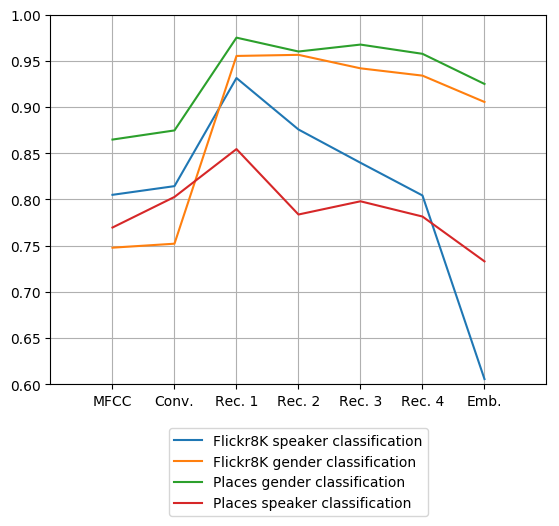
\includegraphics[scale=0.8]{images/gender-speaker-classification.png}\\
	\caption{\label{table:gender-speaker-classification} F1-scores for each experiment.  }
\end{figure}

\begin{figure}[h!]
	\centering
	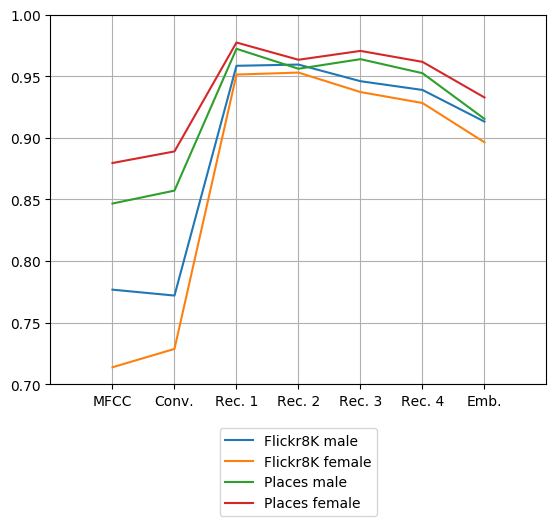
\includegraphics[scale=0.8]{images/gender-bias.png}\\
	\caption{\label{table:gender-bias} F1-scores for gender in both the Places and Flickr8K dataset.  }
\end{figure}

\newpage	
	

% CHAPTER FUTURE WORK AND CONCLUSION
\chapter{Future work and conclusion}\label{chapter:future-work-and-conclusion}

In this chapter I will present future work in \autoref{future-work-and-conclusion:future-work} that is necessary to further examine the extent to which speaker and gender encoding are processed by RNN's based on Visually Grounded Speech. I will also give a final conclusion based on the results presented in \autoref{chapter:experiments} and \autoref{experiments:discussion}.

\section{Future work}\label{future-work-and-conclusion:future-work}

In thesis I used strongly supervised learning to classify speakers by training the linear model with labels of each speaker. By using a Gradient Reversal layer \cite{ganin2016domain} the representation of the speaker can be weakened so that the model is trained and evaluated with less supervision. It would be interesting to see how this affect the performance scores of each layer in each dataset. \\

I mentioned in \autoref{experimental-setup:stratification} that I didn't had any time left to stratify the experiments for speaker identification. Unstratified train and test set could potentially explain why the pattern is less clear in the test set. In future work it is therefore important to research how this limitation affect the performance.

\section{Conclusion}\label{future-work-and-conclusion:conclusion}

In this thesis I presented novel research on the prevalence of gender and speaker encoding in Recurrent Neural Networks based on Visually Grounded Speech signals. To examine how gender encoding involves in this type of Neural Network, it was necessary label all speakers manually into male and female classes. The averaged values of the hidden activations for each layer of the trained Recurrent Neural Network constructed in \cite{ChrupalaGA17} were used. For each layer these values were fed to a linear classifier to determine to what extent encoding of speaker and gender are notable. Various parameters were tried with help of Grid Search to find the optimal score for each layer. After classification on the Flickr8K dataset, the same procedure was applied to the Places dataset to see how the neural network handles a dataset which has longer audio records. Inspired by other research I also decided to examine whether the neural network suffers from any consistent performance differences between males and females. \\

Based on the results in \autoref{chapter:experiments} and \autoref{experiments:discussion}, I conclude that in general the hypothesis is confirmed. Especially taken the F1-scores of the training set into consideration, speaker and gender encoding are most prevalent in the first few layers of the recurrent neural network. The differences are however less notable when you look to the specifics of each experiment. For example, gender encoding in the Flickr8K dataset is slightly more notable in the second recurrent layer than in the first recurrent layer. Moreover, performance on test set for speaker encoding in the Places dataset has a sharp drop in the second recurrent layer although this is not consistent with the results from the training set and accuracy scores. \\

For encoding of males and females the best results were achieved in the Places dataset in all layers. Contrary to gender encoding, speaker encoding follows a different pattern namely that encoding of speakers achieve the best results in the Flickr8K dataset. Comparing encoding of gender and speaker identity the most notable finding is that the prevalence of speaker encoding descends more quickly through the recurrent layers than gender encoding. \\

Research on gender bias revealed that although there are differences for gender classification in both datasets, this is most likely caused by the representation of the data.

\bibliographystyle{apacite}
\bibliography{sources}

\begin{appendices}
\chapter{Accuracy scores for experiments}\label{accuracy-scores-for-experiments}

\begin{figure}[h!]
	\centering
	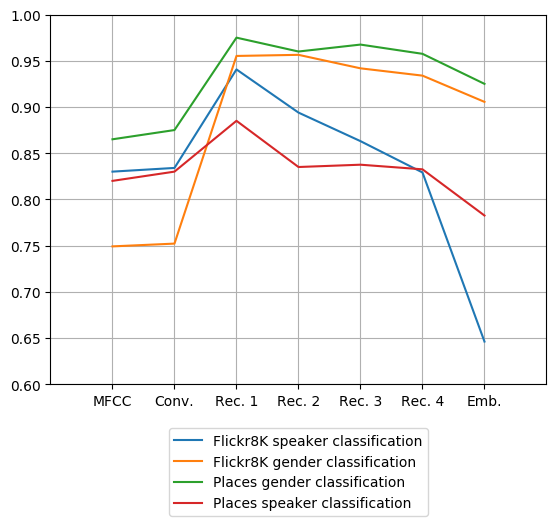
\includegraphics[scale=0.5]{images/gender-speaker-classification-accuracy.png}\\
	\caption{\label{table:gender-speaker-classification-accuracy} Accuracy scores for each experiment.  }
\end{figure}

\begin{figure}[h!]
	\centering
	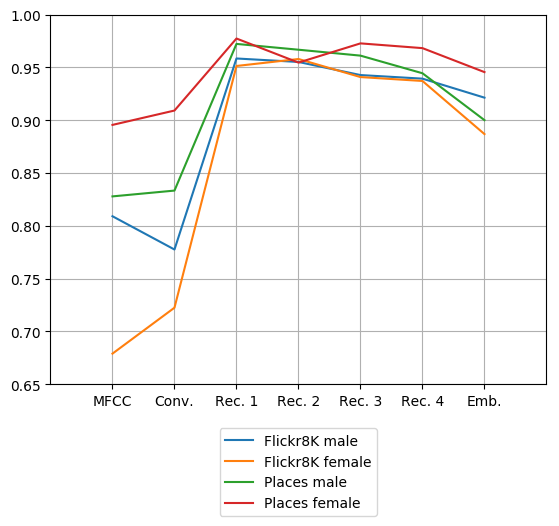
\includegraphics[scale=0.5]{images/gender-bias-accuracy.png}\\
	\caption{\label{table:gender-bias} Accuracy scores for gender in both the Places and Flickr8K dataset.  }
\end{figure}

\chapter{Difference between training and test scores}\label{appendix:difference-between-training-and-test-scores}

\begin{table}[H]
\begin{center}
\begin{tabular}{|l|r|l|l|l|l|}
\hline              & \bf Training F1-score & \bf Test F1-score & \bf Difference  \\ \hline
\bf MFCC            & 0.800                 & 0.8049            & 0.0113 \\
\bf Convolutional   & 0.803                 & 0.8143            & 0.0113 \\ 
\bf Recurrent 1     & 0.925                 & 0.9313            & 0.0063 \\
\bf Recurrent 2     & 0.871                 & 0.8756            & 0.0046 \\
\bf Recurrent 3     & 0.816                 & 0.8396            & 0.0236 \\
\bf Recurrent 4     & 0.773                 & 0.8042            & 0.0312 \\
\bf Embedding       & 0.580                 & 0.6055            & 0.0255 \\
\hline
\end{tabular}
\end{center}
\caption{\label{table:exact-difference-flickr8k-speaker} Exact difference (test - training = difference) in F1-score between prediction on the training and test set for the Flickr8K speaker identification experiment.  }
\end{table}

\begin{table}[H]
\begin{center}
\begin{tabular}{|l|r|l|l|l|l|}
\hline              & \bf Training F1-score & \bf Test F1-score & \bf Difference  \\ \hline
\bf MFCC            & 0.757                 & 0.7477            & -0.0093 \\
\bf Convolutional   & 0.765                 & 0.7520            & -0.0130 \\ 
\bf Recurrent 1     & 0.949                 & 0.9552            & 0.0062 \\
\bf Recurrent 2     & 0.938                 & 0.9564            & 0.0184 \\
\bf Recurrent 3     & 0.929                 & 0.9418            & 0.0128 \\
\bf Recurrent 4     & 0.919                 & 0.9339            & 0.0149 \\
\bf Embedding       & 0.896                 & 0.9054            & 0.0094 \\
\hline
\end{tabular}
\end{center}
\caption{\label{table:exact-difference-flickr8k-gender} Exact difference (test - training = difference) in F1-score between prediction on the training and test set for the Flickr8K gender identification experiment.  }
\end{table}

\begin{table}[H]
\begin{center}
\begin{tabular}{|l|r|l|l|l|l|}
\hline              & \bf Training F1-score & \bf Test F1-score & \bf Difference  \\ \hline
\bf MFCC            & 0.779                 & 0.7695            & -0.0095 \\
\bf Convolutional   & 0.812                 & 0.8026            & -0.0094 \\ 
\bf Recurrent 1     & 0.866                 & 0.8544            & -0.0116 \\
\bf Recurrent 2     & 0.778                 & 0.7836            & 0.0056 \\
\bf Recurrent 3     & 0.774                 & 0.7979            & 0.0239 \\
\bf Recurrent 4     & 0.775                 & 0.7814            & 0.0064 \\
\bf Embedding       & 0.695                 & 0.7329            & 0.0379 \\
\hline
\end{tabular}
\end{center}
\caption{\label{table:exact-difference-places-speaker} Exact difference (test - training = difference) in F1-score between prediction on the training and test set for the Places speaker identification experiment.  }
\end{table}

\begin{table}[H]
\begin{center}
\begin{tabular}{|l|r|l|l|l|l|}
\hline              & \bf Training F1-score & \bf Test F1-score & \bf Difference  \\ \hline
\bf MFCC            & 0.897                 & 0.8647            & -0.0323 \\
\bf Convolutional   & 0.897                 & 0.8746            & -0.0224 \\ 
\bf Recurrent 1     & 0.974                 & 0.9750            & 0.001 \\
\bf Recurrent 2     & 0.965                 & 0.9600            & -0.0065 \\
\bf Recurrent 3     & 0.965                 & 0.9675            & 0.0025 \\
\bf Recurrent 4     & 0.966                 & 0.9575            & -0.0085 \\
\bf Embedding       & 0.951                 & 0.9249            & -0.0261 \\
\hline
\end{tabular}
\end{center}
\caption{\label{table:exact-difference-places-gender} Exact difference (test - training = difference) in F1-score between prediction on the training and test set for the Places gender identification experiment.  }
\end{table}

\end{appendices}

\end{document}
